\chapter{Introduction}
% Approximately 1000 words
% Cycling:
    % Its benefits & its limitations
    % How interactions between drivers and cyclists are currently managed and how that impacts on safety

% How driver psychology should be studied and encouraged in comparison to how it is currently managed

% What is the current situation of how we deal with cyclists in a road safety environment
Vulnerable road users (VRUs), those users who are not protected by the bodywork of a vehicle, are not a majority of those using Irish roads \citep{constantProtectingVulnerableRoad2010}. In 2019 they represented some 15\% of annual journeys on the road network and a significantly smaller proportion of kilometers traveled \citep{departmentoftransportTransportTrends20202020}. However, they are disproportionally represented in Irish crash statistics with 25\% of fatalities in the same year being VRUs \citep{rsaProvisionalReviewFatal2021}. This headline fatality figure also fails to represent the hundreds of injuries that both do and don't get reported to An Garda Síochána (AGS). A publication published by the Road Safety Authority (RSA) details that "the number of injured child cyclists recorded in Irish hospital data is more than six times higher than in records kept by AGS" and that the overall number of cyclists hospitalised was nearly 2.5 times the figures reported by the Gardaí \citep{castelloSeriousInjuriesPedal2023}.

% Address why cycling is to be encouraged
Ireland has among the highest per capita emissions in the EU. Per capita in 2022, Ireland emitted 13.09 kt of CO\textsubscript{2} equivalent greenhouse gasses; the third highest in the EU \citep{eeaEEAGreenhouseGases2024}. Of this, transportation represents 19.1\% and while the CO\textsubscript{2} intensity of private car use is steadily decreasing, it still represents some 40\% of transportation emissions \citep{walshEnergyIreland20202021}. Research into Ireland's transport habits undertaken by the \citet{ntaNationalHouseholdTravel2022}, has discovered that a majority of trips (63\%) taken in Dublin City \& suburbs and close to half of national trips (49\%) are less than 5km in length. These are journeys lengths who's modal shares have been effectively occupied by sustainable modes in countries, like the Netherlands, which actively encourage them \citep{tonCyclingWalkingDeterminants2019}.

\begin{figure}[hbt!]
    \centering
    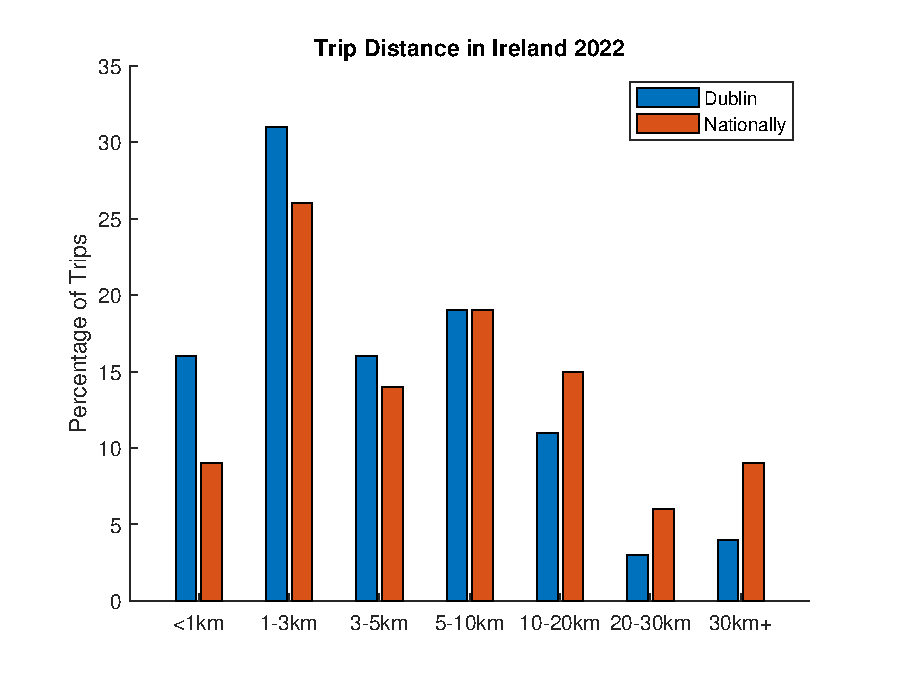
\includegraphics[width=0.60\linewidth]{figures/Irish_trip_distance.eps}
    \caption{Proportion of Trip Distances Nationally and in Dublin \citep{ntaNationalHouseholdTravel2022}}
    \label{fig:TripDistances}
\end{figure}

Cycling has clear and well understood benefits to the environment, health, business, governmental capital and current infrastructure spending and synergies with other sustainable transport modes \citep{fraserCyclingTransportPublic2011,kagerCharacterisationReflectionsSynergy2016, dehartogHealthBenefitsCycling2010}. A pivotal study describing a robust cost-benefit analysis used in Copenhagen concluded that per kilometer, cycling has a cost to society less than a sixth that of motoring \citep{gosslingTransportTransitionsCopenhagen2015}. Due to these factors cycling is is well regarded as a critical piece of the sustainable network of interventions that will be required to address the climate crisis by de-carbonising transportation.

% Address that we are pushing for better/effective infrastructure
As a result of these clear benefits governmental policy has shifted in recent years to have a greater emphasis on driving a modal shift to cycling from private car use. However, a frequently citied barrier to this modal shift is danger both perceived and actual. While it is well understood that the most effective measures to reduce both fatalities and causalities is the introduction of segregated cycling infrastructure there has been an under-delivery relative to Government targets \cite{}. In conjunction with this there has been widespread criticism that the current approach of the Road Safety Authority (RSA) has been sorely lacking in the promotion \& facilitation of this most effective intervention. Instead, the RSA has repeatedly focused their efforts on a number of campaigns to try influence both driver and cyclist behaviour \citep{nugentCyclistsPedestriansAre2015, mcgreevyRoadCyclistsWe2024, rsaCyclistsCampaignRoad2022}.

The effectiveness of these public information campaigns is difficult, if not impossible to measure. However, in the absence of fully segregated infrastructure as situations exist where interaction between cyclist and motorists is inevitable there is some merit in examining what are the factors that influence driver perception and decision making during these interactions.

% Why can this framework of decision neuroscience be used to determine the
Decision neuroscience (DN) is a method of examining human decision making through the application of neuroscience. It can be used to 

Driver psychology has been studied in the past as a method of determining, quantify and reducing the risks associated with driving \cite{}.